\documentclass[
    parskip=half, 
    twoside=false,
    twocolumn=true,
    fontsize=12pt,
]{scrarticle}
\usepackage{xcolor}
\definecolor{seeblau}{HTML}{00A9E0}
\definecolor{seegrau}{HTML}{9AA0A7}

\definecolor{seeblau1}{HTML}{CCEEF9}
\definecolor{seeblau2}{HTML}{A6E1F4}
\definecolor{seeblau3}{HTML}{59C7EB}
\definecolor{seeblau4}{HTML}{00A9E0}
\definecolor{seeblau5}{HTML}{008ECE}


\usepackage{graphicx}
\usepackage{amsmath}
\usepackage{subcaption}
\usepackage{wrapfig}
\usepackage[english]{babel}
\usepackage{blindtext}
\usepackage{microtype}
\usepackage{siunitx}
\usepackage[utf8]{inputenc}
\usepackage{csquotes}
\usepackage{nicefrac}
\usepackage[T1]{fontenc}
\usepackage{amsfonts}
\usepackage{amssymb}
\usepackage{tikz}
\usepackage{parskip}

\usepackage{libertinus, libertinust1math}
\usepackage[sfdefault]{biolinum}
\usepackage{roboto}

\setkomafont{disposition}{\normalfont\sffamily}

% set margins
\usepackage{geometry}
\geometry{
	a4paper,
	left=2.5cm,
	right=2.5cm,
	top=2.5cm,
	bottom=2.5cm
}

% not recommended with KOMA-script
% make table of contents sans-serif
% \usepackage{tocloft}
% \renewcommand\cftchappagefont{\normalfont}
% \renewcommand\cftchapfont{\normalfont}
% \renewcommand\cftchappresnum{\bfseries}
% \renewcommand\cftchapaftersnum{}
% \renewcommand{\cftchapfont}{\sffamily}
% \renewcommand{\cftsecfont}{\sffamily}
% \renewcommand{\cftsubsecfont}{\sffamily}
% \renewcommand{\cftchappagefont}{\sffamily}
% \renewcommand{\cftsecpagefont}{\sffamily}
% \renewcommand{\cftsubsecpagefont}{\sffamily}

% caption
\usepackage{caption}
\captionsetup{
	% font={sf},
	labelfont={sf, bf, color=seeblau},
	labelsep=quad,
	labelformat=simple,
}

% links
\usepackage{hyperref}
\hypersetup{
	colorlinks=true,
	linkcolor=seeblau,
	citecolor=seeblau,
	urlcolor=seeblau,
	% hidelinks=true
}

% bibliography
\usepackage[
	style=numeric-comp, % comp = compressed 4,5,6,7 -> 4-7
	sorting=none,		% Sort by appearance
	% autocite = superscript,
	% backref=true,
	hyperref=true,
	url=true,
	maxbibnames=100
]{biblatex}

\usepackage{float}
% \floatplacement{figure}{h}
% \floatplacement{table}{H}

% loosen float placement rules
\renewcommand{\topfraction}{0.8}
\renewcommand{\bottomfraction}{.8}
\renewcommand{\textfraction}{0.1}
\renewcommand{\floatpagefraction}{.9}
% make floats less likely to be placed on a separate page
\setcounter{totalnumber}{9}
\setcounter{topnumber}{9}
\setcounter{bottomnumber}{9}

% decrease space between floats and text
\setlength{\textfloatsep}{0.25cm}
\setlength{\floatsep}{0.25cm}

% decrease space after disposition
\RedeclareSectionCommands[
	afterskip=1px
]{section, subsection, subsubsection}

\usepackage{adjustbox}

\usepackage{datetime}
\newdateformat{dotdate}{
	\twodigit{\THEDAY}.\twodigit{\THEMONTH}.\THEYEAR
}
\newdateformat{monthyeardate}{%
  \monthname[\THEMONTH] \THEYEAR}


% header and footer
\usepackage[
  markcase=noupper
]{scrlayer-scrpage}% activates pagestyle scrheadings automatically
\clearpairofpagestyles
\setkomafont{pageheadfoot}{\normalfont\sffamily}
\setkomafont{pagenumber}{\normalfont\sffamily}
% \chead*{\color{seegrau} Draft \dotdate\today}
\ofoot*{\pagemark}
\ohead*{\rightmark}


\usepackage{ifthen}
\newcommand{\markieren}[4]{
	\ifthenelse{\equal{#1}{}}{}{\adjustbox{padding=3pt, bgcolor=seeblau1, margin=-1pt}{\strut{\sffamily\robotoMedium{#1}}}\\}
  \ifthenelse{\equal{#2}{}}{}{\adjustbox{padding=3pt, bgcolor=seeblau2, margin=-1pt}{\strut{\sffamily\robotoMedium{#2}}}\\}
	\ifthenelse{\equal{#3}{}}{}{\adjustbox{padding=3pt, bgcolor=seeblau3, margin=-1pt}{\strut{\sffamily\robotoMedium{#3}}}\\}
	\ifthenelse{\equal{#4}{}}{}{\adjustbox{padding=3pt, bgcolor=seeblau4, margin=-1pt}{\strut{\sffamily\robotoMedium{#4}}}}
}


\begin{document}

\title{Modular Tracking}
\author{Leon Oleschko}
\date{\dotdate\today}

\twocolumn[{%
    \sffamily
    \huge
    \markieren{}{}{Modular Tracker}{following a ping pong ball}
    \vspace{.5 cm}\\
    \normalsize
    Leon Oleschko\\
    \dotdate\today
    \vspace{.5 cm}\\
    \normalfont
    \begin{abstract}
        Real-time detection, tracking, and control are fundamental to applications in robotics and automation. This project presents a modular, high-speed camera tracking system designed to explore detection, tracking, and control strategies by following a ping pong ball during gameplay. The system combines a Raspberry Pi Camera V2, stepper motors, and a Raspberry Pi 5, achieving real-time tracking at \SI{200}{Hz} through a modular Python-based software stack. The modular design and user-friendly interface make the system accessible for experimentation and learning, while its performance under controlled conditions demonstrates its potential for applications in robotics, sports analytics, and beyond.
    \end{abstract}
    \bigskip
}]

\subsection*{Introduction}
Real-time object tracking is a core challenge in computer vision and robotics. Moving a camera to track a ping pong ball during gameplay creates an interesting platform to explore and evaluate detection, tracking, and control strategies. This is due to its unique combination of steady ballistic flight interrupted by rapid, complex bounces at high speeds.

To simplify the exploration of different strategies, the system is designed with modularity and accessibility in mind. Each component is built around high-level concepts, enabling users to experiment without requiring an in-depth engineering background.


\section{Methods}
The system is designed to track a ping pong ball in real time by moving a camera dynamically. To achieve this, the project is broken down into modular components, each addressing a specific aspect of the tracking process. 

\subsection*{Hardware}
\begin{figure}
    \centering
    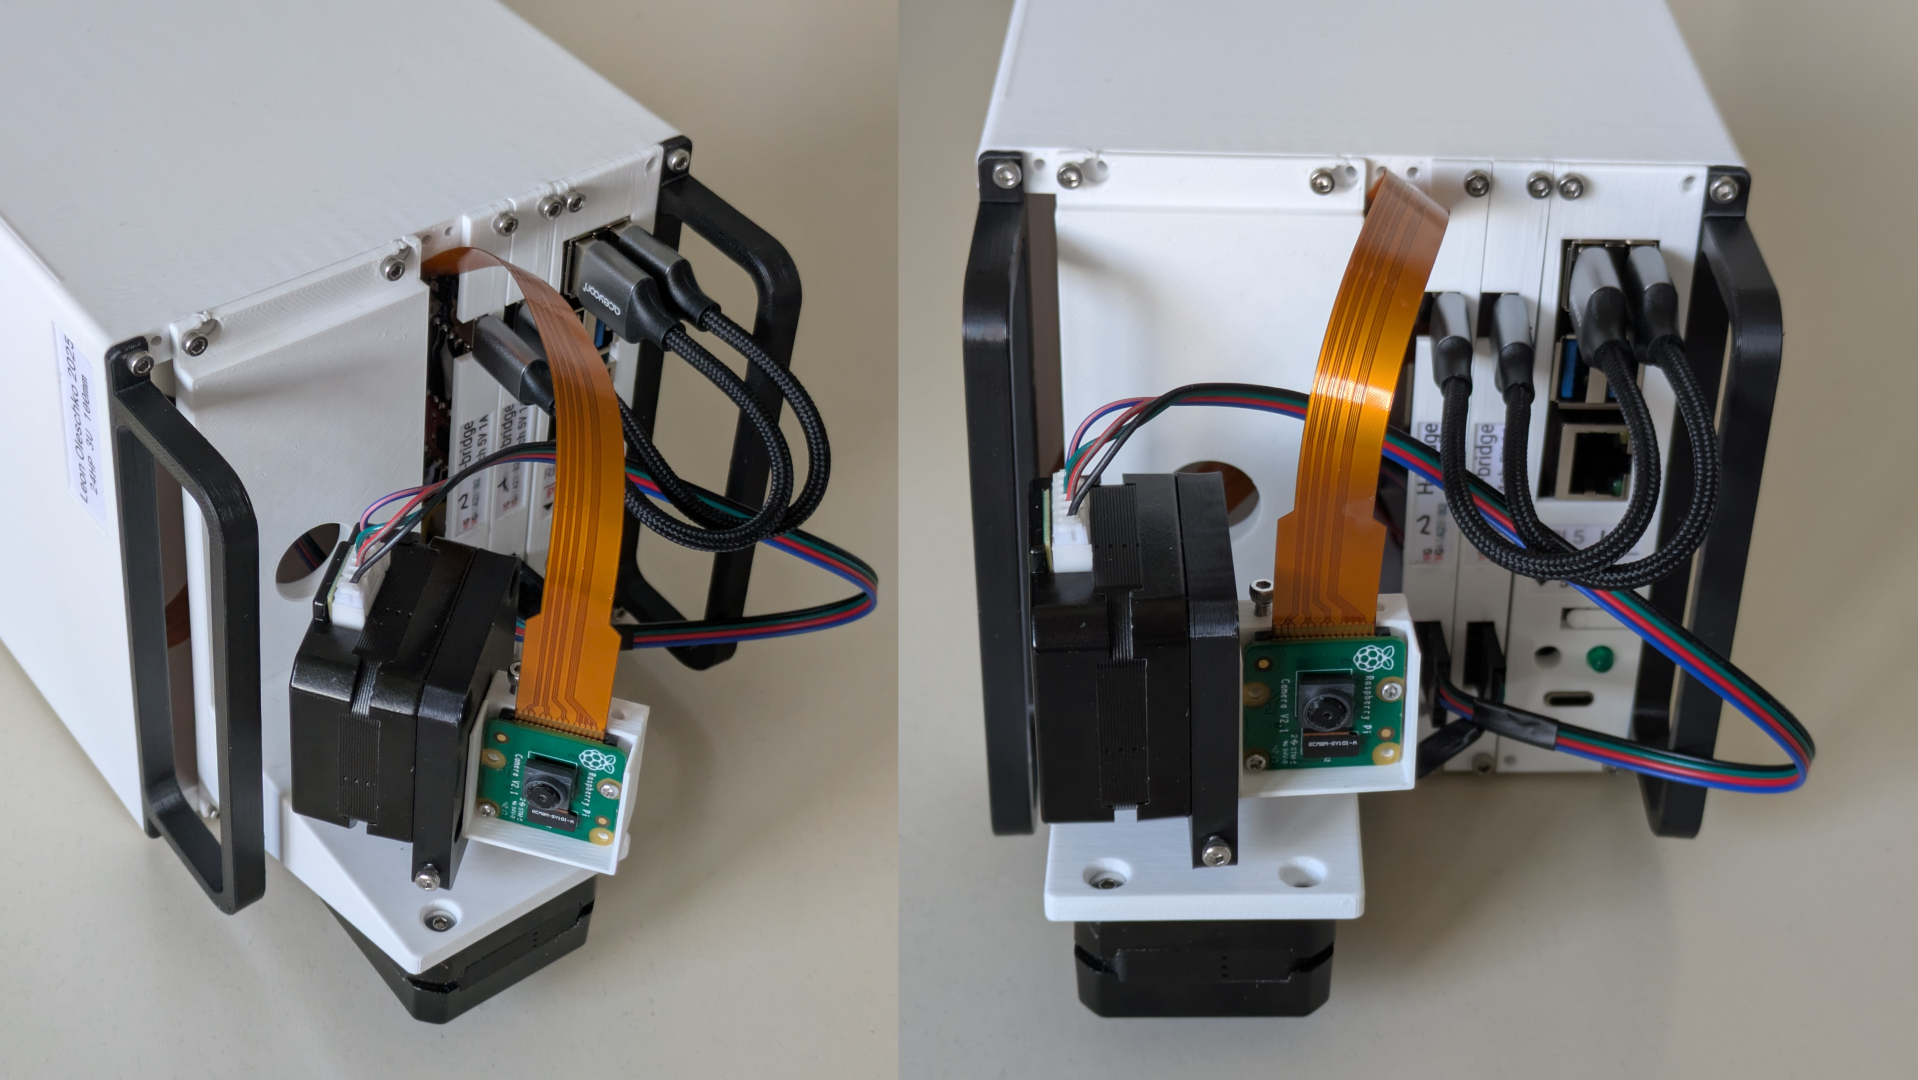
\includegraphics[width=0.5\textwidth]{../../hardware/assembly.png}
    \caption{Mechanical assembly of all components.}
    \label{fig:assembly}
\end{figure}
The hardware components consists of a camera, motors, motor controllers and a processing computer.\\
The modules are designed as subrack modules and can be assembled as shown in \autoref{fig:assembly}.


For the camera a Raspberry Pi Camera V2 is used, as with the \href{https://github.com/raspberrypi/picamera2}{picamera2} software stack it supports a framerate of \SI{200}{Hz}.
A normal \SI{30}{Hz} USB Webcam was tested to be not sufficient.\\
To move the camera 2 common stepper motors are mounted perpendicularly.
They are driven with field oriented controllers with the \href{https://simplefoc.com/}{SimpleFOC} firmware stack.
They are connected to the control computer using the Universal Serial Bus (USB).\\
The chosen computer is a Raspberry Pi 5.

To power the components \SI{9}{V}~\SI{3}{A} from a USB-C power supply are converted to a \SI{5}{V}~\SI{5}{A} bus for the computer and another \SI{5}{V}~\SI{3}{A} bus for the motors.
Additionally the startup of the computer and the motors is staggered.
This was necessary to achieve stable operation.

\subsection*{Software}
The software architecture is designed to be modular, ensuring flexibility and ease of experimentation. It is split into a camera module, detector module, and motor module, with plans to add a tracker module and controller module in the future. Each module can be independently evaluated, modified, or replaced, allowing users to experiment with different algorithms and configurations without affecting the entire system.

The camera module configures the camera into a high frame rate mode and fetches new frames.

The detector identifies the center of the ping pong ball in the image by comparing each pixel's color $I(x,y)$ to a predefined reference color $R$ in the Hue Saturation Luminance (HSL) color space.
Testing showed that HSL outperformed Luminance-AB (LAB).
For each pixel, a weight $w$ is computed:
$$w = \exp\left(- \frac{(I(x,y)-R)^2}{\sigma}\right)$$
Where $\sigma$ is the standard deviation of each channel in a reference image of the ball.
This function emphasizes pixels closely matching the reference color while exponentially reducing the influence of outliers.
The color channels are then summed to get one weight for each pixel.
The location of the ball is determined by finding the position of the maximum weight in the image.\\
This process is efficiently implemented using \href{https://numpy.org/}{numpy}, allowing the detector to process an downsampled $80\times 60$ pixel frame in \SI{3.6}{ms}.
This high-speed performance is critical for real-time tracking, ensuring the system can keep up with the fast-moving ball during gameplay.

The tracker evaluates the detector's maximum weight $w_\text{max}$ to determine if the detection is valid.
Using hysteresis, it compares $w_\text{max}$ to two thresholds $T_\text{heigh} > T_\text{low}$.
If $\omega_\text{max}>T_\text{heigh}$ it is valid; if $\omega_\text{max}<T_\text{low}$ it is invalid.
For values In between $T_\text{low}<\omega_\text{max}<T_\text{heigh}$ the pervious state is kept.\\
This hysteresis-based approach ensures robust and smooth tracking, even under challenging conditions. 

The motors are moved based on the error, which is the angle between the detected ball position and the center of the camera's field of view. This error is scaled by a constant factor, producing a control signal that drives the motors. This approach is known as a P-regulator (proportional controller), where the motor response is directly proportional to the error. While simple, this method provides effective and responsive control for keeping the ball centered in the frame.

\section{Results}
The simple detection and tracking approach works smoothly under controlled lighting conditions and with a differently colored background. However, in uncontrolled lighting environments, the threshold for detection must be lowered to maintain sensitivity, which introduces false positives. Despite this limitation, the system demonstrates robust performance in ideal conditions, highlighting its potential for applications where lighting can be managed.

\section{Conclusion}
This project demonstrates the feasibility of a modular, high-speed camera tracking system for following a ping pong ball in real time. By combining a simple yet effective detection algorithm with a proportional controller, the system achieves reliable performance under controlled lighting conditions. The modular design allows for easy experimentation with different strategies, making it a versatile platform for learning and innovation in real-time object tracking.

Future work could focus on improving robustness in uncontrolled lighting environments, such as by incorporating adaptive thresholding or machine learning-based detection methods. Additionally, expanding the system to include more advanced control strategies, like PID control or predictive tracking, could further enhance performance. The platform also holds potential for applications beyond ping pong, such as in robotics, sports analytics, or automated surveillance, making it a valuable tool for both education and research.

\end{document}